\section{Experimental setup}

Here we discuss the experimental setup used to produce the results. The
results here act both as a proof of principle of the data space estimators
presented in this paper but also as part of a suite of methodological
validation tools, see also the "future tests" \cite{Cruz_Martinez_2021},
used to
understand the PDF uncertainties of the upcoming NNPDF4.0 set of PDFs.
For the purpose of understanding how the results here were produced, we
will briefly describe the key features of the NNPDF4.0 methodology,
but refer the reader to NNPDF4.0 for a full discussion on how these
methodological choices were made, and the impact on performing PDF fits
to experimental data.

\subsection{Neural network parton distribution functions}

Using neural networks to fit PDFs has been discussed many times in previous
NNPDF publications, see for example \cite{nnpdf30, Ball_2017}. A new
feature of NNPDF4.0 will be that, for the default fit performed in the
evolution basis, a
single neural network parameterises all 8 PDF flavours $\{ g, \Sigma, V, V_3, V_8, T_3, T_8, c^+ \}$
at the initial scale. The PDF for a single flavour $j$, at the initial scale
$Q_0 = 1.65 {\rm GeV}$ is given by
\begin{equation}
    f_j(x, Q_0) = NN(x, \ln x | \modelvec)_j * x^{1-\alpha_j} * (1-x)^{\beta_j},
\end{equation}
where $\alpha$ and $\beta$ are the preprocessing exponents, which control the
PDF behaviour at $x \to 0$ and $x \to 1$ respectively and
$NN(x, \ln x | \modelvec)_j$ is the
$j^{\rm th}$ output of the neural network, which takes $x$ and $\ln x$ as input.
As discussed in Sec.~\ref{sec:fit-reps}, an ensemble of models is fitted, each
one is an MAP estimator of the corresponding pseudo-data it is fitted on. Unlike
in the case of the linear model, the parameters of the neural network cannot be
found analytically and instead an optimization algorithm is used to try and
find the parameters which maximise the likelihood. In principle, the preprocessing
exponents can also be varied during the fit analogously to the neural network
parameters, such as in \cite{Carrazza_2019}, or they can be randomly selected
from a predetermined range as is done in previous NNPDF releases,
for example \cite{Ball_2017}. There are clearly many choices with respect
to hyperparameters, the discussion of how these choices have been made is
beyond the scope of this paper and left to the full NNPDF4.0 release
\cite{NNPDF40}. A brief summary of the hyperparameters used to produce results
presented in this paper are provided in Tab.~{tab:Hyperparams}.

\begin{table}
    \begin{tabular}[h]{c|c}
        {\rm bf TODO} & {\bf FILL}
    \end{tabular}
\end{table}

Finally, the parton distributions themselves are not compared directly with data.
Instead the observables quantities are obtained by performing convolutions with
the PDFs, as discussed in \ref{eq:DISExample}. In practice the observables are
obtained by convoluting the PDFs with FastKernel tables, presented in
\cite{Ball_2010,Bertone_2017}, for each data point. The convolution depends
on the process type of the observable, for DIS-like observables, such as in
Eq.~\ref{eq:DISExample}, the convolution is performed with a single PDF. For
hadronic observables the convolution is performed between two PDFs.

\subsection{Closure test setup}

As input to the closure test, a single replica was drawn randomly from
a previous NNPDF fit to experimental data. We refer to this as the underlying
law and the corresponding predictions the true observable values. An example
of the gluon input is provided in Fig.~\ref{fig:InputGluonPDF}. In principle
any function could be used as underlying law, however it makes sense to
use a realistic input.

\begin{figure}
    \centering
    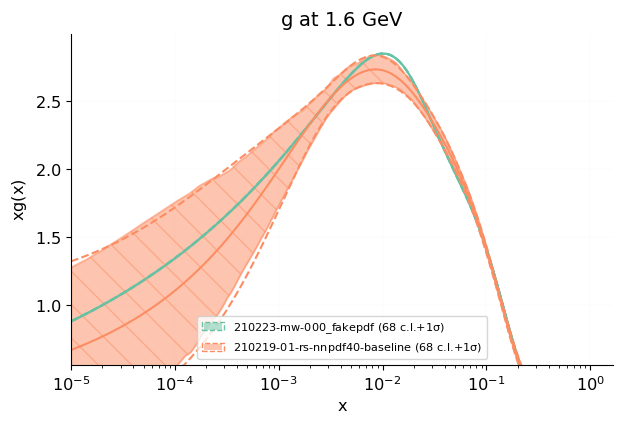
\includegraphics[width=0.6 \textwidth]{plot_pdfs_g.png}
    \caption{The green line is the input underlying law for the gluon PDF,
    which is sampled from the ensemble from a fit to data. The 68\% confidence
    interval is plotted for those replicas as the orange band.}
    \label{fig:InputGluonPDF}
\end{figure}


The observables used in the fits are a subset of the full NNPDF4.0 dataset.
For convenience,
we chose to fit the PDFs on a variant of the NNPDF3.1 dataset used in
\cite{Ball_2018}, which is described in detail in a study of the determination
of the strange PDF \cite{Faura_2020}. The datasets used in the calculation of
statistical estimators are the new datasets which will be included in NNPDF4.0,
and are summarised in Tab.~\ref{tab:summarise_new_data}, but not discussed in detail.

\begin{table}[h!]
    \begin{center}
    \resizebox{0.6\textwidth}{!}{\begin{tabular}{llll}
        \toprule
        {} & Training fraction & C-factors & Other fields \\
        Dataset                                &                   &           &              \\
        \midrule
        ATLASPHT12                             &                 - &       QCD &            - \\
        ATLASPHT15                             &                 - &       QCD &            - \\
        ATLAS\_SINGLETOP\_TCH\_R\_7TEV             &                 - &       QCD &            - \\
        ATLAS\_SINGLETOP\_TCH\_DIFF\_7TEV\_T\_PT     &                 - &       QCD &            - \\
        ATLAS\_SINGLETOP\_TCH\_DIFF\_7TEV\_T\_RAP    &                 - &       QCD &            - \\
        ATLAS\_SINGLETOP\_TCH\_DIFF\_7TEV\_TBAR\_PT  &                 - &       QCD &            - \\
        ATLAS\_SINGLETOP\_TCH\_DIFF\_7TEV\_TBAR\_RAP &                 - &       QCD &            - \\
        ATLAS\_SINGLETOP\_TCH\_R\_8TEV             &                 - &       QCD &            - \\
        ATLAS\_SINGLETOP\_TCH\_DIFF\_8TEV\_T\_PT     &                 - &       QCD &            - \\
        ATLAS\_SINGLETOP\_TCH\_DIFF\_8TEV\_T\_RAP    &                 - &       QCD &            - \\
        ATLAS\_SINGLETOP\_TCH\_DIFF\_8TEV\_TBAR\_PT  &                 - &       QCD &            - \\
        ATLAS\_SINGLETOP\_TCH\_DIFF\_8TEV\_TBAR\_RAP &                 - &       QCD &            - \\
        ATLAS\_SINGLETOP\_TCH\_R\_13TEV            &                 - &       QCD &            - \\
        ATLAS\_2JET\_7TEV\_R06                    &                 - &  QCD, EWK &            - \\
        ATLAS\_2JET\_7TEV\_R04                    &                 - &  QCD, EWK &            - \\
        ATLAS\_WP\_JET\_8TEV\_PT                   &                 - &       QCD &            - \\
        ATLAS\_WM\_JET\_8TEV\_PT                   &                 - &       QCD &            - \\
        ATLAS\_WP\_JET\_8TEV\_PTJ                  &                 - &       QCD &            - \\
        CMS\_SINGLETOP\_TCH\_TOT\_7TEV             &                 - &       QCD &            - \\
        CMS\_SINGLETOP\_TCH\_R\_8TEV               &                 - &       QCD &            - \\
        CMS\_SINGLETOP\_TCH\_R\_13TEV              &                 - &       QCD &            - \\
        CMS\_2JET\_7TEV                          &                 - &  QCD, EWK &            - \\
        CMS\_2JET\_3D\_8TEV                       &                 - &  QCD, EWK &            - \\
        \bottomrule
        \end{tabular}}
\end{center}
    \caption{
        {\bf TODO: update!!}
        Summary of the new processes, out of sample data used to compute the
        statistical estimators.
    }
    \label{tab:summarise_new_data}
\end{table}

The choice of fitted datasets is
considered unimportant, one could consider splitting the data into training
and test in a way which considered kinematic coverage rather than this
naive chronological splitting. Alternatively, since the data is generated from
the theory predictions produced by the input underlying law, one could even
produce completely artificial data using a different set of FK tables. From a
practical standpoint, using the NNPDF3.1 dataset and validating on the newly
included
datasets in 4.0 allowed us to validate the PDF uncertainities on data outside
of the kinematic coverage of data included in the fit. Furthermore, the data estimators
only give us local information on the PDF uncertainties and it seems
logical to split the data in this way since the results seem more applicable to
the reality of how the PDFs end up being used.

We then generate 30 different sets of experimental central values
(or L1 data), as discussed in Sec.~\ref{sec:closure-test-intro}, for the
fitted 3.1-like dataset.
Each set of experimental central values was then
fitted following NNPDF4.0 methodology \cite{NNPDF40},
producing 40 pseudo-data replicas.